\documentclass[varwidth]{standalone}
\usepackage[portrait,paperwidth=30cm,
paperheight=40cm,
textwidth=26cm,
textheight=36cm]{geometry}
\usepackage{bera}
\usepackage[T1]{fontenc}
\usepackage[swedish]{babel}
\usepackage[utf8]{inputenc}
\usepackage{amsmath}
\usepackage{bm}
\usepackage{tikz}
\usepackage{pgfplots}
\usepackage{tikz}
\usepackage{tkz-euclide}
\usepackage{pgfgantt}
\usetikzlibrary{decorations.pathmorphing}
\usetikzlibrary{patterns}
\usetikzlibrary{arrows}
\usepackage{pgfplots}
\usepackage{CJKutf8}
\pgfplotsset{compat=1.10}
\usetikzlibrary{shapes.geometric,arrows,fit,matrix,positioning}
\begin{document}
\newcommand{\radie}[0]{1mm}
\begin{center}
\begin{figure}
\centering
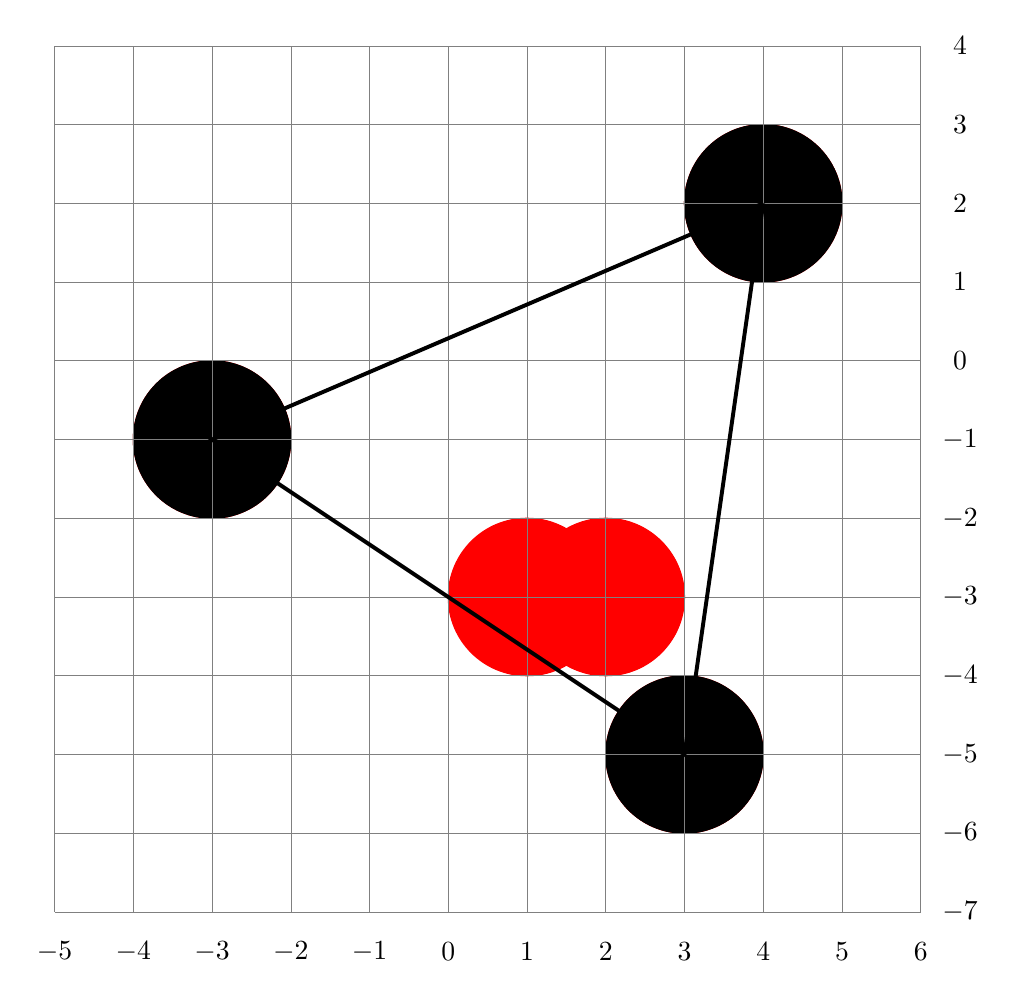
\begin{tikzpicture}
\draw [red,fill=red] (4.000000,2.000000) circle(\radie);
\draw [red,fill=red] (2.000000,-3.000000) circle(\radie);
\draw [red,fill=red] (3.000000,-5.000000) circle(\radie);
\draw [red,fill=red] (-3.000000,-1.000000) circle(\radie);
\draw [red,fill=red] (1.000000,-3.000000) circle(\radie);
\draw [black,fill=black] (4.000000,2.000000) circle(\radie);
\draw [black,fill=black] (3.000000,-5.000000) circle(\radie);
\draw [black,fill=black] (-3.000000,-1.000000) circle(\radie);
\draw[step=10mm,gray,very thin] (-5,-7) grid (6,4);
\node at (-5,-7.500000) {$-5$};
\node at (-4,-7.500000) {$-4$};
\node at (-3,-7.500000) {$-3$};
\node at (-2,-7.500000) {$-2$};
\node at (-1,-7.500000) {$-1$};
\node at (0,-7.500000) {$0$};
\node at (1,-7.500000) {$1$};
\node at (2,-7.500000) {$2$};
\node at (3,-7.500000) {$3$};
\node at (4,-7.500000) {$4$};
\node at (5,-7.500000) {$5$};
\node at (6,-7.500000) {$6$};
\node at (6.500000,-7) {$-7$};
\node at (6.500000,-6) {$-6$};
\node at (6.500000,-5) {$-5$};
\node at (6.500000,-4) {$-4$};
\node at (6.500000,-3) {$-3$};
\node at (6.500000,-2) {$-2$};
\node at (6.500000,-1) {$-1$};
\node at (6.500000,0) {$0$};
\node at (6.500000,1) {$1$};
\node at (6.500000,2) {$2$};
\node at (6.500000,3) {$3$};
\node at (6.500000,4) {$4$};
\draw [line width = 0.5mm, black] (4.000000,2.000000) -- 
(3.000000,-5.000000) -- 
(-3.000000,-1.000000) -- 
(4.000000,2.000000);
\end{tikzpicture}
\end{figure}
\end{center}
\end{document}
